\section{HDF - Hybrid-Dimensional-Formulation}
\begin{wrapfigure}{l}{6cm}
  \centering
  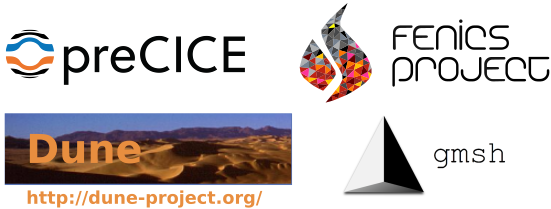
\includegraphics[width=6cm]{figures/0a_hdf_packages.png}
  \caption{Packages used to develop Hybrid-Dimensional Framework}
  \label{fig:hdf_packages}
\end{wrapfigure}
The Hybrid-Dimensional-Formulation results in a numerically strongly coupled system of governing equations. Different numerical strategies, namely the weak/staggered and strong/monolithic coupling schemes have been implemented in course of this project to solve the interaction between fluid flow and deformation of the surrounding porous matrix. Dependent on the method different technical requirements are demanded from the numerical framework. Hence for each one of the two coupling strategies an individual numerical framework has been chosen to guarantee numerical efficiency.

For the strongly coupled scheme high performance has been ensured by choosing the Distributed and Unified Numerics Environment (DUNE) \cite{dune24:16} to monolithically build and solve the global system of governing equations. The Dune implementation is based on modern C++ programming techniques to provide a unique combination of highly efficient and flexible code by providing a common interface at a very low overhead for various mesh based methods. Combined with the generalized discretization module PDELab \cite{dune:pdelab} the basis for Finite Element calculations of the implemented solver has been built. Nevertheless, extensive work on the existing framework has been performed in order to allow the integration of zero-thickness elements; a feature which is not provided by default.

The staggered algorithm of the weak coupling scheme allows for calculations on different numerical domains. Efficient numerical implementation combined with a versatile way to handle continuously varying boundary conditions provided by the FEniCS computing platform \cite{AlnaesBlechta2015a} form the basis of the developed solver. Since the coupling between both domains is numerically strong an implicit coupling iteration is required. The Precise Code Interaction Coupling Environment (preCICE) \cite{preCICE} provides an easily accessible interface for parallel communication between existing solvers allowing for non-conformal discretization of computational domains in combination with a highly developed Quasi-Newton method to guarantee numerical stability.

Discretization for both methods, namely the construction of interface elements and separation of fracture surfaces is a challenging task especially in three dimensions. This challenge has been overcome by an in house meshing tool based on the Gmsh meshing facility \cite{doi:10.1002/nme.2579}.
